

Nektar++ \cite{Mo20Nekt, nektarwebsite} is a framework for solving partial differential equations (PDEs) using the spectral / hp-element method.  
The software contains several different solvers targeting canonical problems in fluid mechanics.  
It is possible to extend the framework by adding new domain-specific solvers; this currently involves low-level coding as there is no DSL.  
Nektar++ is being used in Project \nep\ as the framework for the higher-order solution of fluid equations and currently is being extended to handle plasma fluids.  Data is extracted from Nektar++ simulations by means of \emph{filters} and written to text-based output files.

A small team from UKAEA 
%(Ed Threlfall and Will Saunders) 
attended the three VECMAtk hackathons in Spring 2021.
The goal of the hackathon work was to create the software framework to enable
Nektar++ to use VECMAtk,
and to develop workflows for uncertainty quantification and the creation of
surrogate models.
%The code produced at the hackathons is available in the repository \cite{nektar_vecma_repo}.

\subsection{Software Infrastructure}

The VECMA toolkit wraps around an individual Nektar++ solver to provide non-intrusive UQ (only non-coupled workflows are considered here).  
The toolkit interacts with Nektar++ via the inputs and outputs of the latter, through respectively an \emph{encoder} and a \emph{decoder}; 
these objects can be interchanged to enable different workflows (for example, the relevant quantities of interest (QoIs) are parsed in the decoder). 

\subsection{Uncertainty Quantification}

The initial test problem used the incompressible Navier-Stokes solver of Nektar++ to simulate classical convection: 
a two-dimensional fluid-filled slot with vertical walls maintained at different temperatures; starting with an initial uniform temperature gradient from the hot side to the cold side, the system is time-evolved until a steady state is reached.  
Warmer fluid is subject to an upward buoyancy force, leading to a steady convective cell solution with fluid travelling up the hot side and down the cold one.

In dimensionless form, the equations for fluid velocity $\bf{u}$, temperature $T$ and pressure $p$ are

\begin{eqnarray}
\frac{1}{Pr} \left ( \frac{\partial \bf u}{\partial t} + {\bf u} \cdot \nabla {\bf u} \right ) &=& - \nabla p + Ra \; T \; \hat{{\bf y}} + \nabla^2 {\bf u}\\
\left ( \frac{\partial T}{\partial t} + {\bf u} \cdot \nabla T \right ) &=& \nabla^2 T\\
\nabla \cdot {\bf u} &=& 0.
\end{eqnarray}

Here, the Rayleigh number $Ra$ and the Prandtl number $Pr$ are the governing parameters and are taken to be subject to uncertainty. 

%The QoIs are the Nusselt number, the dimensionless heat flux across the cavity (normalized to the $Ra=0$ solution, which corresponds to the initial data)

%\begin{equation}
%Nu = -\frac{1}{2H} \int_0^H \nabla_x T(x_0,z)+\nabla_x T(x_1,z) dz.
%Nu = \frac{ \int_0^H -\nabla_x T(x_0,y)+\nabla_x T(x_1,y) dy }{ \int_0^H -\nabla_x T(x_0,y)+\nabla_x T(x_1,y) dy \rvert_{Ra=0}}
%\end{equation}

%and also the temperature profile across a horizontal line half-way up the cavity.

The Nektar++ simulations were designed so as to run quickly on a single desktop computer.  
Computational parameters governing accuracy were chosen to give plausible results without detailed analysis of convergence.

\subsubsection{Polynomial chaos expansion}

A square slot was used as a first example; the results follow closely the original investigation in \cite{El65Nume}.  
An example temperature profile over the full domain can be see in Figure \ref{fig:tempfield}.

\begin{figure}[tbp]
\begin{centering}
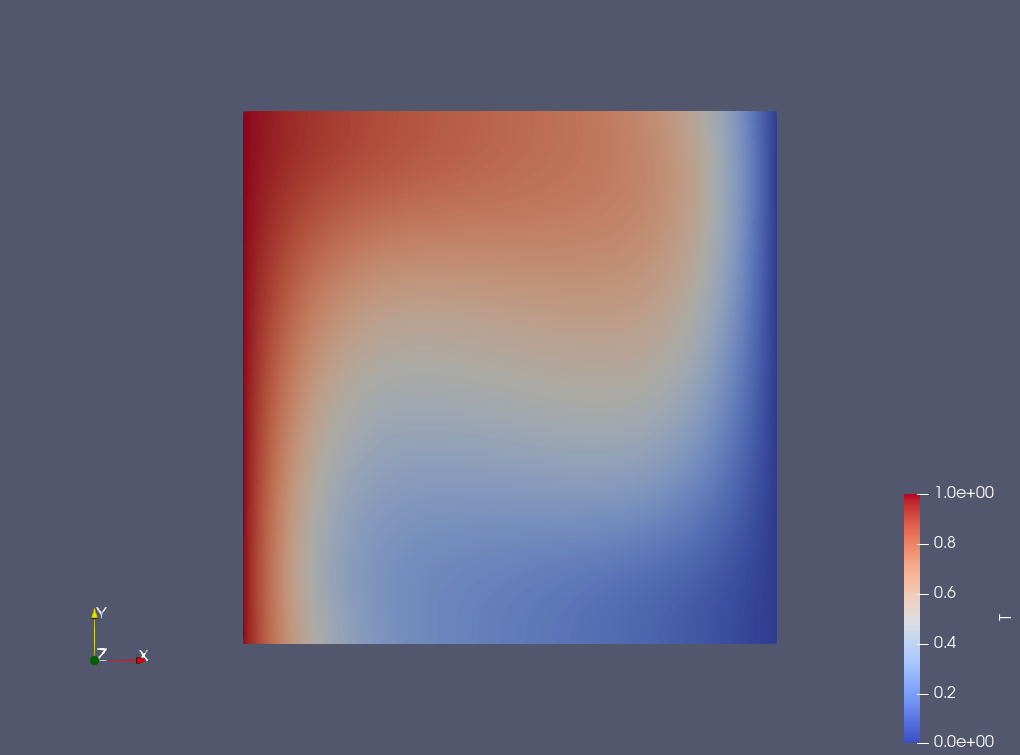
\includegraphics[width=0.5\textwidth]{laminar.png}
\caption{\small Steady-state colour map of dimensionless temperature for $Ra=10^4$, $Pr=1.0$.  The left side is maintained at a temperature one unit higher than the right and a convective cell carries fluid in a clockwise circulation.
\label{fig:tempfield}
}
\par
\end{centering}
\end{figure}

The QoI was the temperature profile $T(x)$ evaluated half-way up the slot, parsed via the decoder \texttt{SlicedHisDecoder} from data extracted using the Nektar++ \texttt{HistoryPoints} filter to record field values at chosen sample points.  %Again, a decoder (\texttt{SlicedHisDecoder}) parses a text file output by Nektar++ and extracts the QoI.
Note that the sample points cannot lie on the vertical boundaries, as the Dirichlet boundary condition enforces constant temperature values there, which causes the analysis to fail (a singular matrix error is reported by VECMA).  
$Pr$ was taken to be in the range $1-10$ (values typical for the gases and liquids commonly investigated in the literature), with a uniform distribution.  
$Ra$ was taken to be in the range $1.0\times 10^4 - 3.2 \times 10^4$ (values consistent with a laminar convective steady state), with a log-uniform distribution.

The polynomial chaos expansion (PCE) produces a fit to the sampled QoI data using a sum over orthogonal polynomials in the input variables, where the orthogonality is defined using the input probability distributions as the measure and the fit is performed by either spectral projection or linear regression.  
The polynomial chaos analysis of EasyVVUQ provides the mean, variance, and standard deviation of the outputs and also the minimum, maximum, median and the $1^{st}$, $10^{th}$, $90^{th}$, and $99^{th}$ percentiles (a useful \texttt{supported\_stats()} routine lists the available statistics).  
Some of these quantities are shown in Figure \ref{fig:temp_profile}, which was generated using a fifth-order PCE.  
Also shown are the first Sobol indices, which show correctly that the uncertainty in the output is dominated by the sensitivity to~$Ra$ in this case; in the regime in question, the effect of varying $Pr$ is small.

\begin{figure}[tbp]
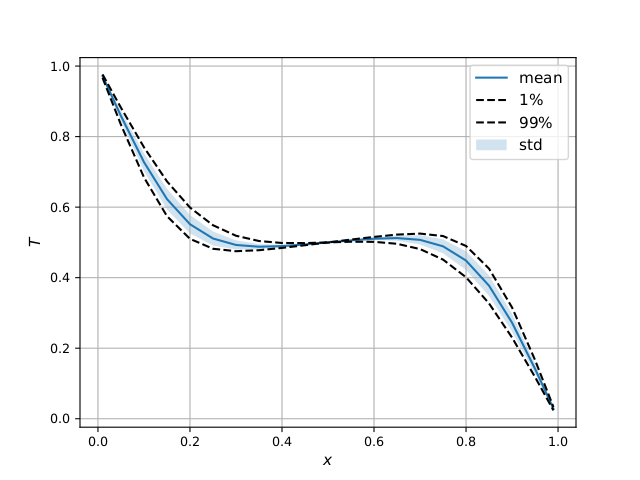
\includegraphics[width=0.5\textwidth]{T_vs_x_mean_ci_nektar.png}
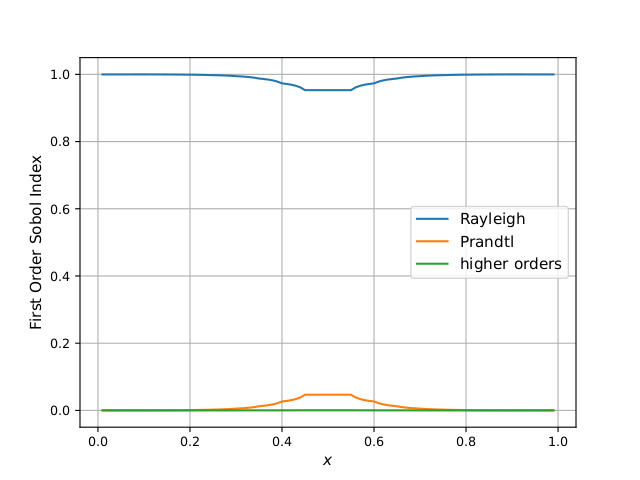
\includegraphics[width=0.5\textwidth]{T_vs_x_sobols_nektar.png}
\caption{%
Mean and confidence intervals (left) and first Sobol indices (right) as a function of position
for the central temperature profile $T(x)$ fitted by a polynomial chaos expansion.  Note that the uncertainty tends to zero in regions where the temperature is 
either fixed (end points) or is constrained by symmetry (centre).  
\label{fig:temp_profile}
}
\end{figure}

\subsubsection{Stochastic collocation}

Stochastic collocation (SC) creates a representation of the QoIs that is exact at the sample points; the solution is a linear combination of sample-point values multiplying Lagrange polynomials at those points.  
The stochastic collocation analysis of EasyVVUQ provides the mean, variance and standard deviation of the outputs.  
The set of available statistics is smaller than for the PCE, but the method is more efficient (as explained earlier in this report).  
The decoder used in the preceding section is switchable between PCE and SC.

\subsection{Surrogate models}

Note that, although it concerns surrogate models, the work in this subsection used EasyVVUQ and not EasySurrogate.

\subsubsection{Polynomial chaos expansion and stochastic collocation}\label{sec:pceasc}

Either of the orthogonal polynomial fit constructed in the polynomial chaos expansion or the Lagrange polynomial fit constructed in the stochastic collocation method can serve as a computationally-inexpensive surrogate for the full model.  
As an example, PCE and SC surrogates for the Nusselt number $Nu$ as a function of $Ra$ and $Pr$ were constructed.  $Nu$ is the dimensionless heat flux across the cavity, normalized to the $Ra=0$ no-convection solution, calculated as

\begin{equation}
%Nu = -\frac{1}{2H} \int_0^H \nabla_x T(x_0,z)+\nabla_x T(x_1,z) dz.
Nu = \frac{ \int_0^H \partial_x T(x_0,y)+\partial_x T(x_1,y) dy }{ \int_0^H \partial_x T(x_0,y)+\partial_x T(x_1,y) dy \rvert_{Ra=0}} \; .
\end{equation}
where $\partial_x$ denotes partial derivative with respect to coordinate~$x$.

The Nusselt number was extracted using a customized filter in Nektar++ and the output file was parsed by a decoder (\texttt{HeatFluxDecoder}) using a simple text processing routine.  
An illustration of the SC and PCE fits (both using fifth-order polynomial expansions) for the simple case of Nusselt number as a function of the Rayleigh number ($Pr=1$) is shown in Figure \ref{fig:nektar_surrogate}.  
The Nusselt number is seen to follow a typical power-law curve.

\begin{figure}[tbp]
\begin{centering}
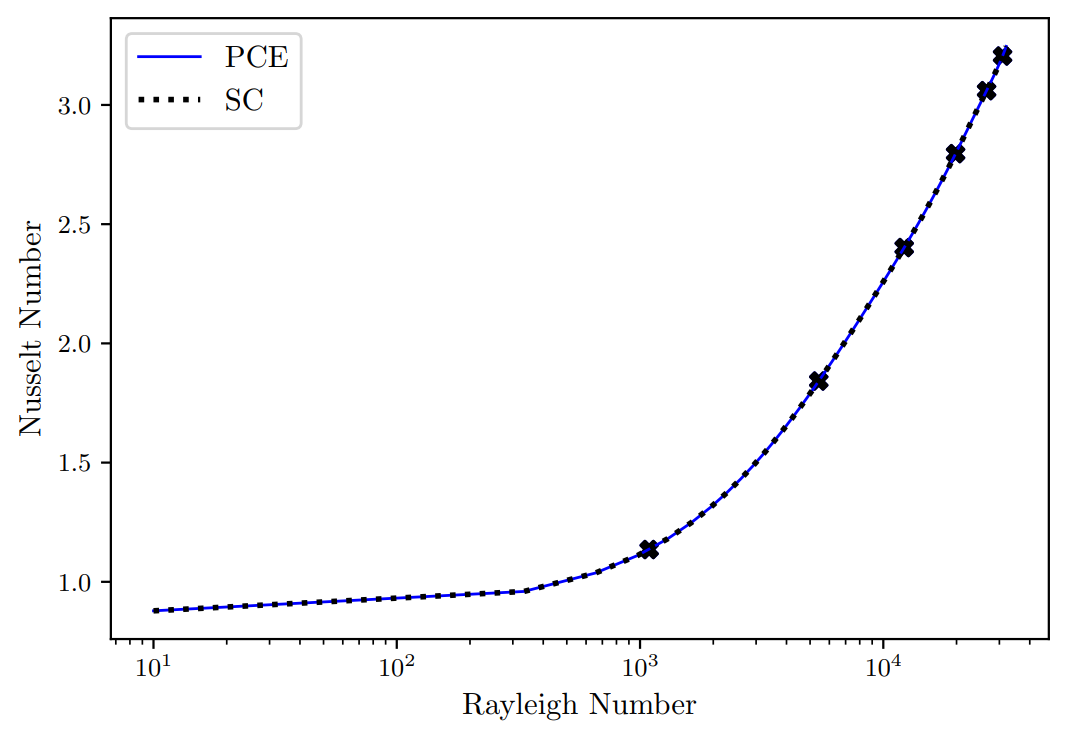
\includegraphics[width=0.5\textwidth]{nektar_surrogate.png}
\caption{\small Polynomial chaos and stochastic collocation surrogates for Nusselt number as a function of Rayleigh number, for Prandtl number $1.0$.
\label{fig:nektar_surrogate}
}
\par
\end{centering}
\end{figure}

\subsubsection{Gaussian process surrogate}

A different set-up, though again using the Nektar++ incompressible Navier-Stokes solver, was used as an initial exploration of the Gaussian process surrogate capability in EasyVVUQ; 
this was a slot $10$ units high and $1$ wide, operating at larger Rayleigh numbers where the flow exhibits a boundary-layer instability with waves moving up the hot wall and down the cold one (illustrated in Figure \ref{fig:wallwavesetc}).  
This gave interesting time series for the maximum temperature near the affected parts of the walls (the lower part of the cold wall was used) and the position of the hottest point.  
These QoIs are of interest in fusion applications as they characterize the hot spots on the wall of a reactor containing hot plasma.  
The time series were extracted over a chosen time window using a customized filter in Nektar++; 
the simulation runs were performed once and the decoder (\texttt{HotSpotDecoder}) was given the ability to read stored simulation data in order to avoid repeating calculations.
In view of the weak dependence on the parameter $Pr$, only the parameter $Ra$ was varied in this activity (values in the range $10^5-10^7$ were used).  
A kernel with zero mean and a Mat\'ern covariance with parameters $\nu=3/2$ and scale $10^7$ were used.

\begin{figure}[tbp]
\begin{centering}
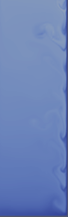
\includegraphics[height=0.6\textheight]{wall_waves.png}\\
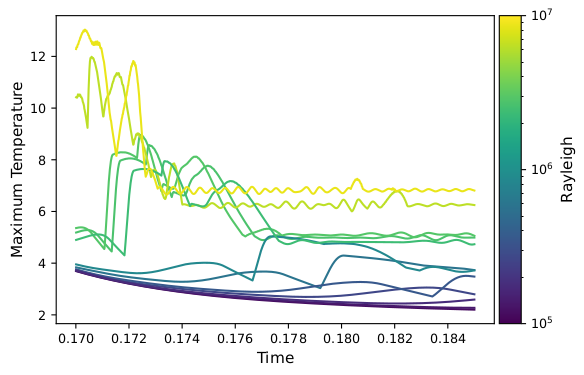
\includegraphics[width=0.4\textwidth]{gp_observed_max_temp.png}
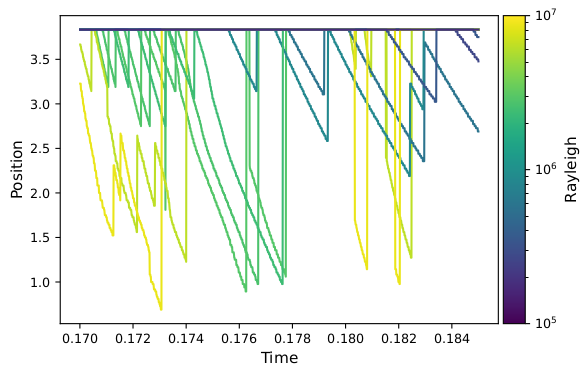
\includegraphics[width=0.4\textwidth]{gp_observed_position.png}
\caption{\small Boundary-layer instability at the cold wall for $Ra=2.3 \times 10^8$ (top). 
The maximum temperature on this part of the wall and also the position of the hottest point are shown as time series (respectively left and right below).
\label{fig:wallwavesetc}
}
\par
\end{centering}
\end{figure}

This investigation was an attempt at finding a surrogate for computations that are more demanding than the laminar convection ones in the preceding section and also concerned a system that exhibits deterministic chaos.
The time series data used to train the Gaussian process is shown in Figure \ref{fig:wallwavesetc}.  
Note that for $Ra$ sufficiently large for the instability to form, temperature maxima enter from the top of the monitored section and proceed downwards until usurped by the next wave.  
For smaller values of $Ra$, the system is quiescent and the time series eventually become constant.
Some sample evaluations of the Gaussian process surrogate away from the sample points can be seen in Figure \ref{fig:GPoutputs}.  It can be seen that the surrogate correctly reproduces the more active nature of the time series for larger values of $Ra$.

\begin{figure}[tbp]
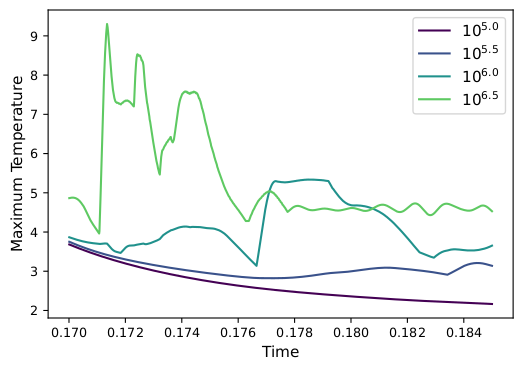
\includegraphics[width=0.5\textwidth]{gp_sample_max_temp.png}
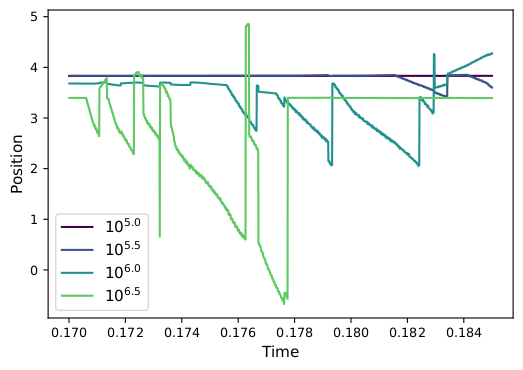
\includegraphics[width=0.5\textwidth]{gp_sample_position.png}
\caption{%
Output of the Gaussian process surrogates for the maximum temperature and the position of the hottest point evaluated at positions away from the sample parameter values.  
\label{fig:GPoutputs}
}
\end{figure}








